\section{Simulation}
\label{sec:simulation}
\textcolor{red}{Use the previous model to calculate the transfer function of the ADC (dout(vin))
and compute the transition voltages of the ADC for a given set of errors.}

\textcolor{red}{Use the model to measure the linearity of the ADC using INL, DNL and FFT.}

\textcolor{red}{Run Monte Carlo analysis of the ADC model to determine the sensitivity of the
ADC to mismatch errors between the different components.}

\textcolor{red}{Introduce specific errors into the values of key capacitors in the array (such as CB, Cdl, etc) and observe the resulting impact in the INL and DNL. Observe and explain the effect of the offset voltage on the ADC transfer function. Also compare the difference between using CB=2 or CB=16/15.}

\textcolor{red}{Present a histogram of the linearity of the ADC resulting from the monte carlo analysis. Run this analysis for different magnitude of random errors in the capacitors. Present the best, worst and average INL and DNL from this analysis.}


Explicar - para comparar com os resultados do paper, na tecnologia $\SI{65}{\nano\meter}$, com $C_u = \SI{6.5}{\femto\farad}$

To test and simulate the ADC transfer function, and since there are no ideal values for the capacitors or any component present in the ADC in study, a Monte Carlo analysis is needed to guarantee a robust implementation to these variations, ensuring a reliable converter.

\subsection{Capacitors value}

Depending on manufacturing specifics, there are different ways to define how the capacitors variation will behave. If the capacitors are built by summing unitary capacitors with independent variations, the variation will decrease. For the Monte Carlo analysis, this was \textbf{not} assumed, the same variation was used for all capacitor sizes.
%First, to test the response of the ADC to the variation of the capacitors values, that respect a normal distribution, with defined variance $\sigma$ of the unit capacitor.

To guarantee a viable result of the Monte Carlo analysis, $20~000$ simulations were executed for all values presented in this report, resulting in the Transfer Functions presented in Figure \ref{fig:ADC_TF_ALLCAPS}.

\begin{figure}[H]

    \centering
    \includegraphics*[width=0.9\textwidth]{Images/ADC_TransFunc_All_Caps_20Ksim_s0011.png}
    \caption{ADC's Transfer function for Capacitor values variation}

    \label{fig:ADC_TF_ALLCAPS}
\end{figure}

Since the ADC in analysis has a resolution of 12 bits, it is not possible to see any result of the Monte Carlo simulation with only the Transfer Functions of all iterations, so it is necessary to analize the INL and DNL errors, shown in Figure \ref{fig:NL_ALLCAPS}

\begin{figure}[H]
    \centering
    \begin{subfigure}[b]{0.8\textwidth}
        \centering
        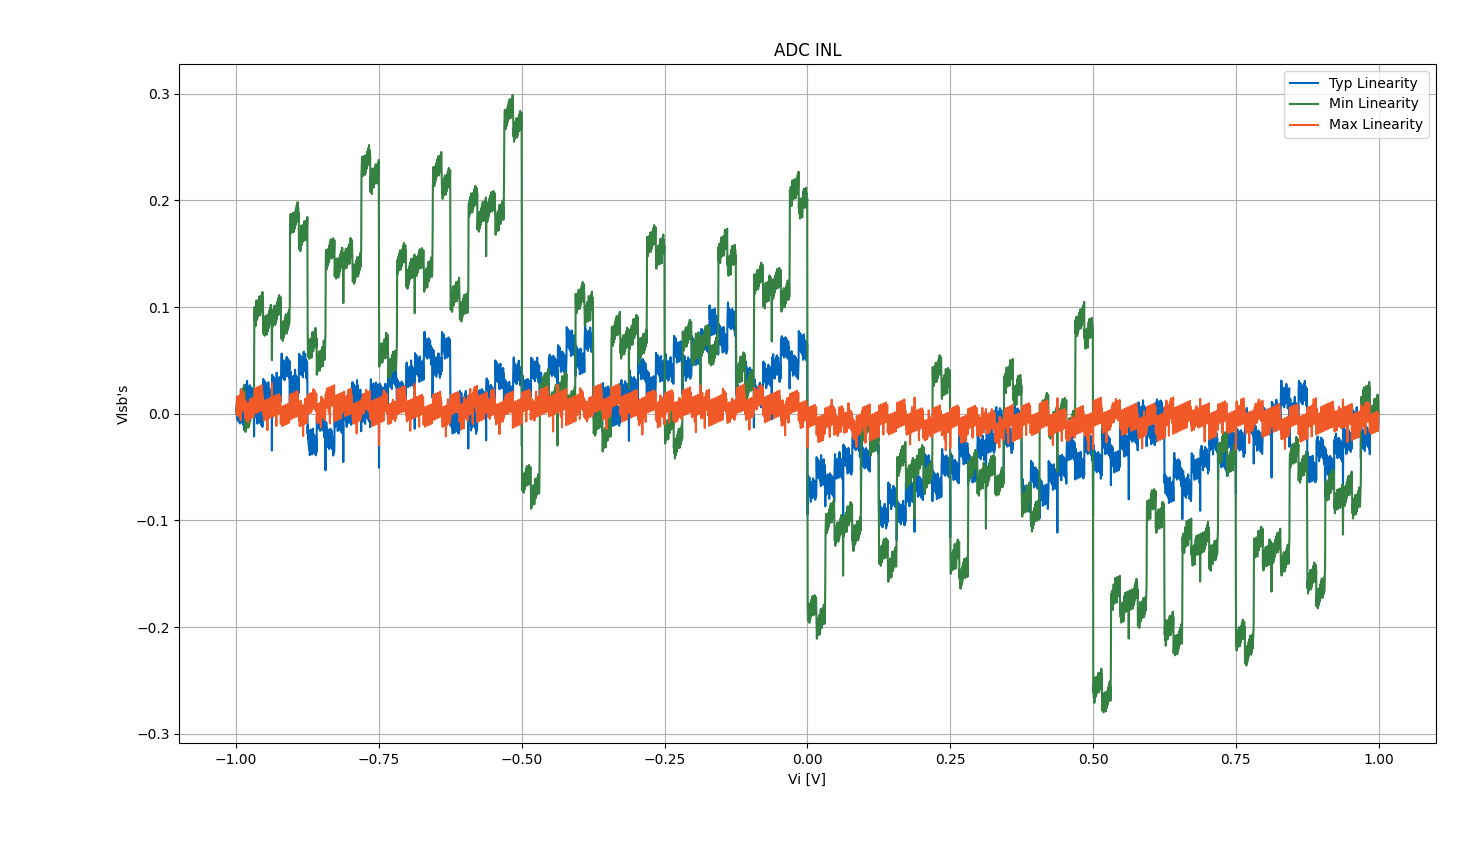
\includegraphics[width=\textwidth]{Images/INL_All_Caps_20Ksim_s0011.png}
        \caption{INL}
        \label{fig:INL_ALLCAPS}
    \end{subfigure}%
    
    \begin{subfigure}[b]{0.8\textwidth}
        \centering
        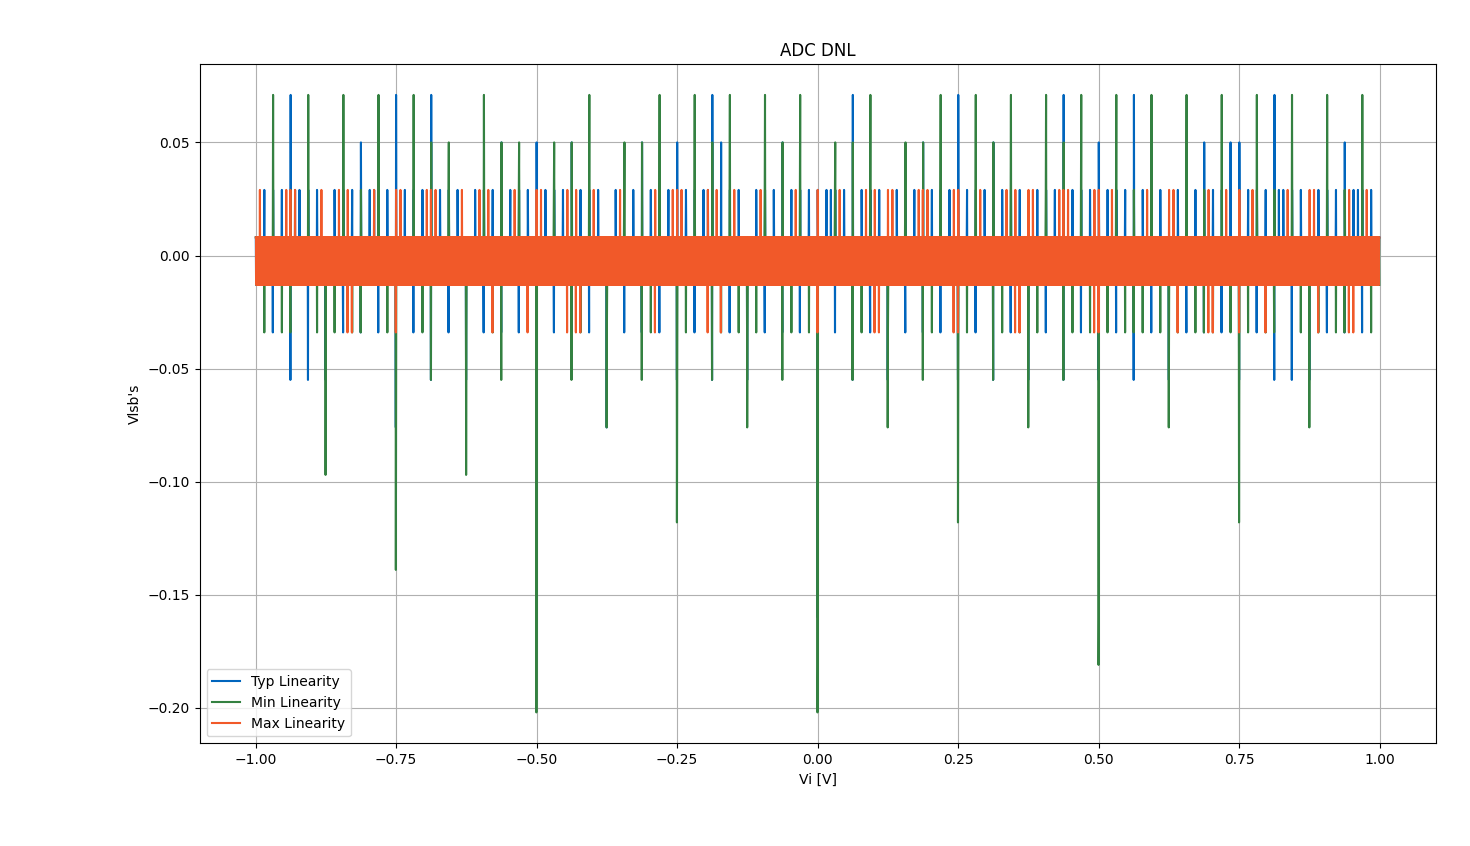
\includegraphics[width=\textwidth]{Images/DNL_All_Caps_20Ksim_s0011.png}
        \caption{DNL}
        \label{fig:DNL_ALLCAPS}
    \end{subfigure}
    \caption{INL and DNL Error for Capacitor values variation}
    \label{fig:NL_ALLCAPS}
\end{figure}

With the INL and DNL, is possible to observe that in the both errors, in the worts case, or minimum linearity value, there are no missing code, since the maximum or minimum value of the INL or DNL passes the value of a single $V_{lsb}$. 

Finally, it is also possible to observe the distributions of the ADC's SNR and Linearity for the simulation carried out in Figures \ref{fig:ADC_SNR_ALLCAPS} and \ref{fig:ADC_LIN_ALLCAPS}, respectively.

\begin{figure}[H]

    \centering
    \includegraphics*[width=0.8\textwidth]{Images/SNR_All_Caps_20Ksim_s0011.png}
    \caption{ADC's SNR Distribution.}
    \label{fig:ADC_SNR_ALLCAPS}
\end{figure}

\begin{figure}[H]

    \centering
    \includegraphics*[width=0.8\textwidth]{Images/LIN_All_Caps_20Ksim_s0011.png}
    \caption{ADC's Linearity Distribution.}

    \label{fig:ADC_LIN_ALLCAPS}
\end{figure}

The distribution of the ADC's SNR is represented by a left-skewed distribution, with a mean value of approximately $\SI{73.85}{\decibel}$, validating the value obtained previously.

Regarding the Linearity distribution, this is represented by a normal distribution, equl to the distribution of the capacitor values, with a mean of $14.25$ bits, approximately, higher than the $12$ bits resolution of the ADC, which means, the resolution presented is supported by the converter.

\begin{comment}

$\sigma = 0.05$, $n_{sim} = 20000$

#############
IMAGENS PRA SIGMA = 0.05

\begin{figure}[H]

    \centering
    \includegraphics*[width=0.8\textwidth]{Images/ADC_TransFunc_All_Caps_20Ksim.png}
    \caption{ADC's Transfer function. \textcolor{red}{Melhorar titulo}}

    \label{fig:ADC_TF_ALLCAPS}
\end{figure}

\begin{figure}[H]
    \centering
    \begin{subfigure}[b]{0.8\textwidth}
        \centering
        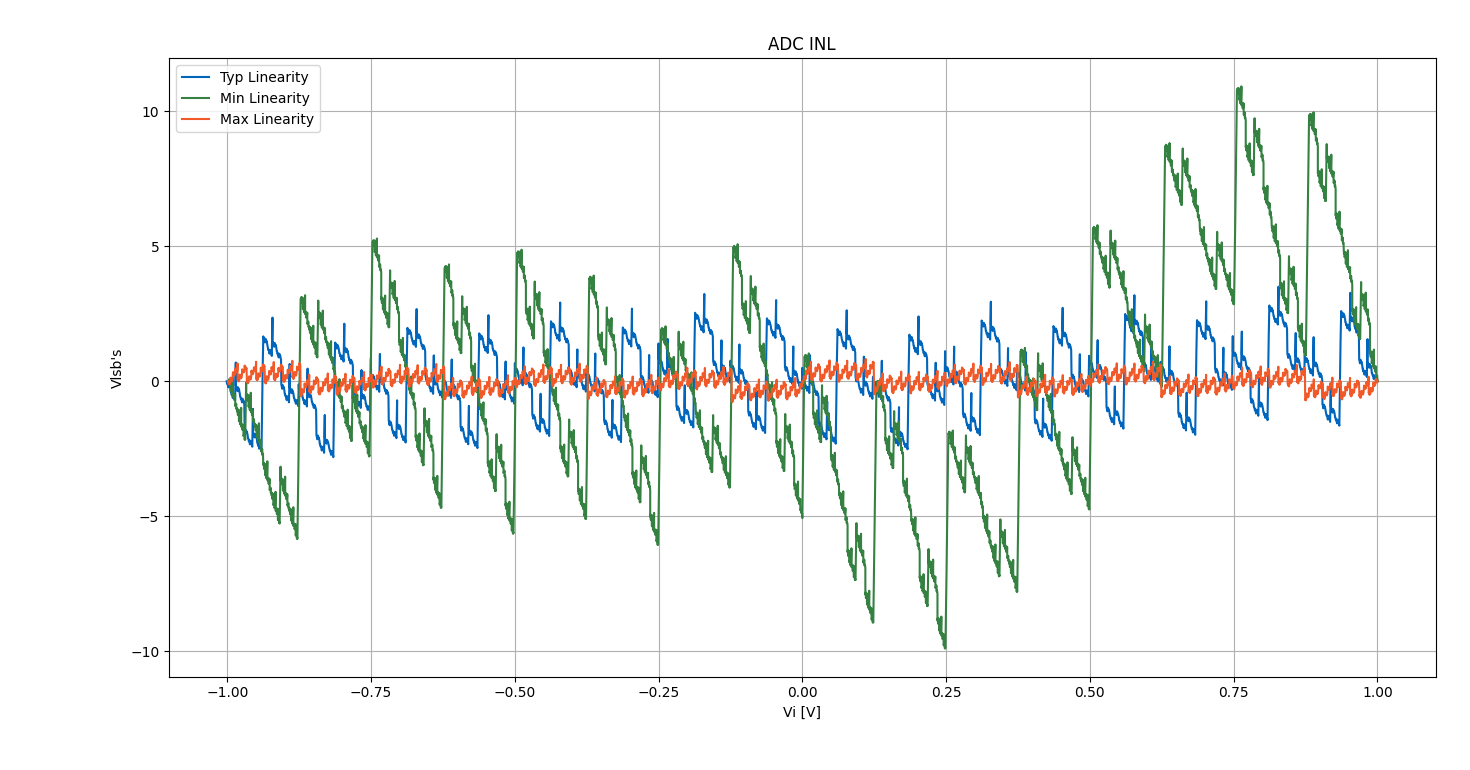
\includegraphics[width=\textwidth]{Images/INL_All_Caps_20Ksim.png}
        \caption{INL}
        \label{fig:INL_ALLCAPS}
    \end{subfigure}%
    
    \begin{subfigure}[b]{0.8\textwidth}
        \centering
        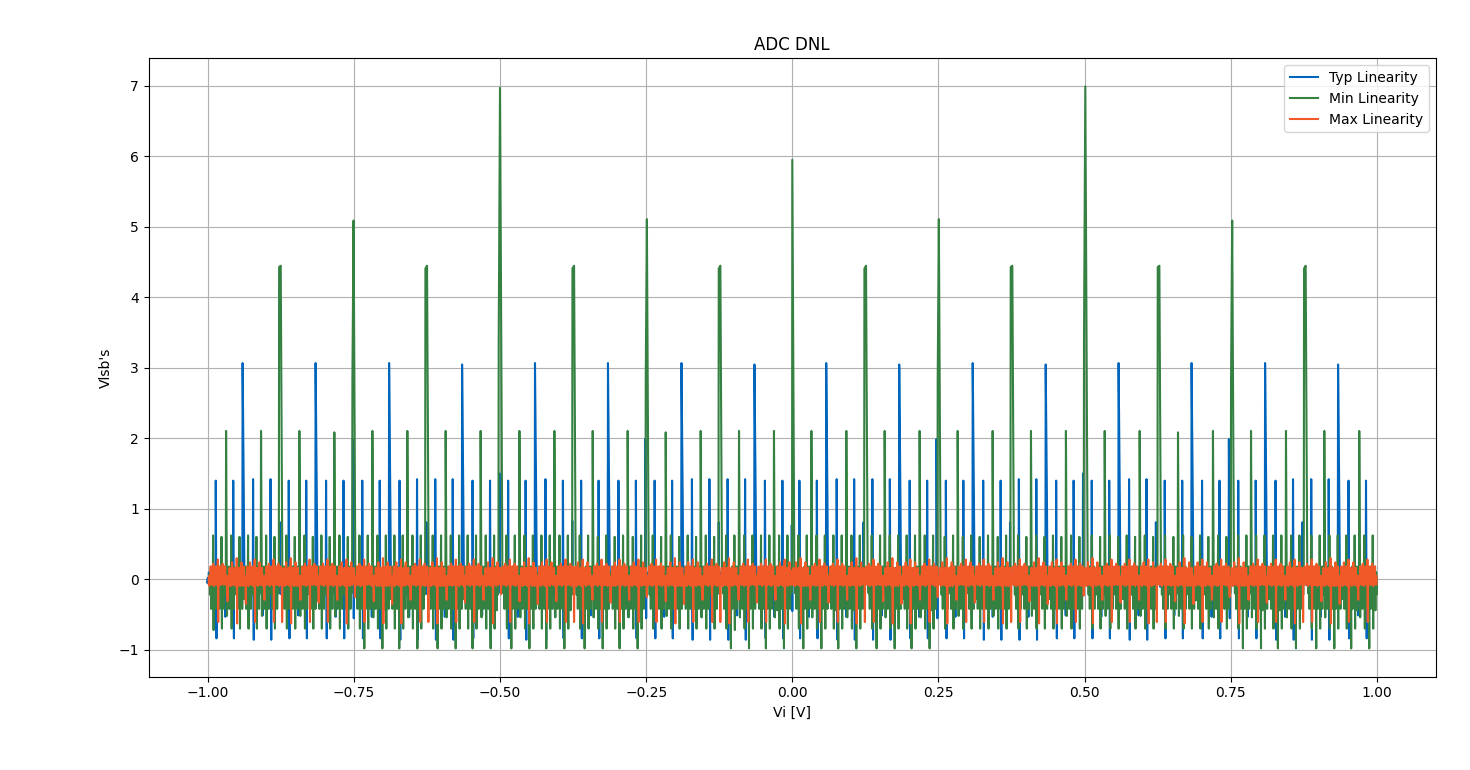
\includegraphics[width=\textwidth]{Images/DNL_All_Caps_20Ksim.png}
        \caption{DNL}
        \label{fig:DNL_ALLCAPS}
    \end{subfigure}
    \caption{INL and DNL Error \textcolor{red}{Lado a Lado ou uma em cima da outra?}}
    \label{fig:NL_ALLCAPS}
\end{figure}

\begin{figure}[H]

    \centering
    \includegraphics*[width=0.8\textwidth]{Images/SNR_All_Caps_20Ksim.png}
    \caption{ADC's SNR Distribution. \textcolor{red}{Melhorar titulo}}
    \label{fig:ADC_SNR_ALLCAPS}
\end{figure}

\begin{figure}[H]

    \centering
    \includegraphics*[width=0.8\textwidth]{Images/Vlsb_All_Caps_20Ksim.png}
    \caption{ADC's VLSB Distribution. \textcolor{red}{Melhorar titulo}}
    \label{fig:ADC_VLSB_ALLCAPS}
\end{figure}

\begin{figure}[H]

    \centering
    \includegraphics*[width=0.8\textwidth]{Images/LIN_All_Caps_20Ksim.png}
    \caption{ADC's Linearity Distribution. \textcolor{red}{Melhorar titulo}}

    \label{fig:ADC_LIN_ALLCAPS}
\end{figure}

\end{comment}



\subsection{ $V_{\text{Offset}}$ }


To test the influence of the offset voltage variation in the comparator, a sweep in these value was made, between the values of $V_{\text{Offset}} \in [\SI{-10}{\milli\volt},\SI{10}{\milli\volt}]$. The resulting ADC's Transfer Functions are displayed in Figure \ref{fig:ADC_TF_Offset}.



\begin{figure}[H]

    \centering
    \includegraphics*[width=0.8\textwidth]{Images/ADC_TransFunc_Voffset.png}
    \caption{ADC's Transfer Function for different $V_{offset}$.}

    \label{fig:ADC_TF_Offset}
\end{figure}

To better see the result of the variationn of the offset voltage, the INL and DNL were calculated, resulting in the graphics shown in Figure \ref{fig:NL_Voffset}.


\begin{figure}[H]
    \centering
    \begin{subfigure}[b]{0.8\textwidth}
        \centering
        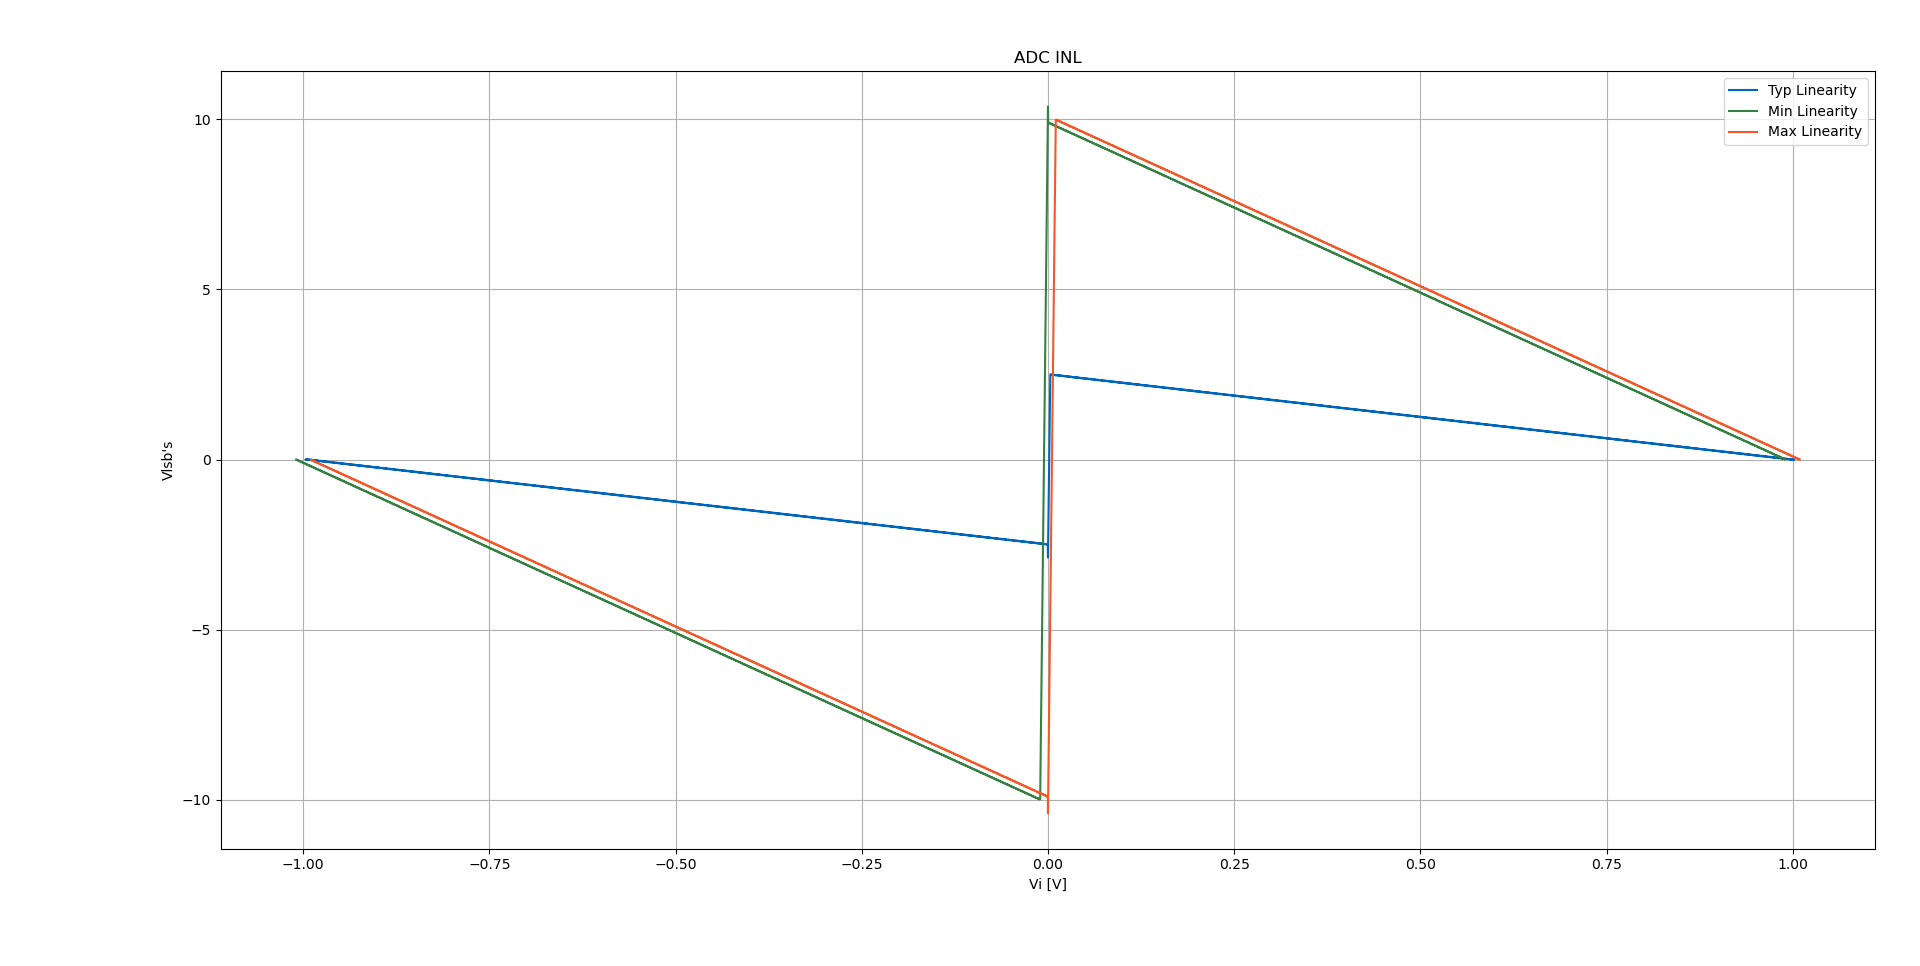
\includegraphics[width=\textwidth]{Images/INL_Voffset.png}
        \caption{INL}
        \label{fig:INL_Voffset}
    \end{subfigure}%
    
    \begin{subfigure}[b]{0.8\textwidth}
        \centering
        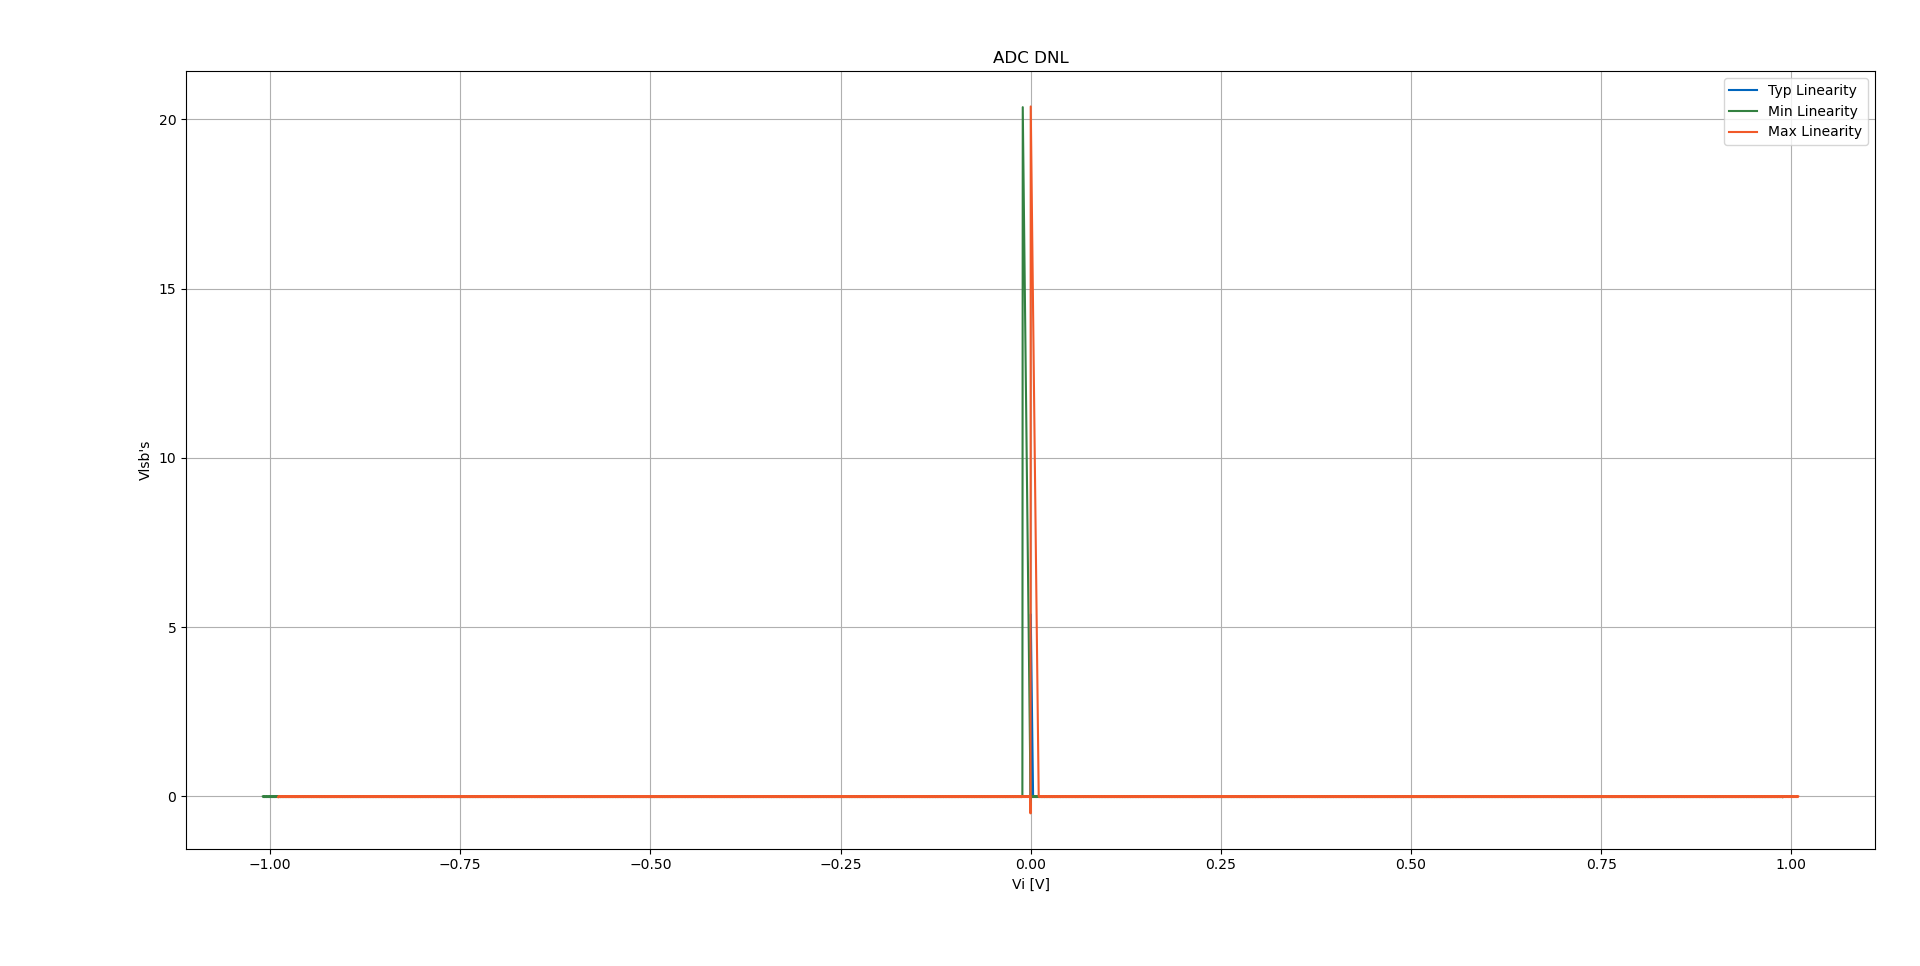
\includegraphics[width=\textwidth]{Images/DNL_Voffset.png}
        \caption{DNL}
        \label{fig:DNL_Voffset}
    \end{subfigure}
    \caption{INL and DNL Error for $V_{offset}$ variation}
    \label{fig:NL_Voffset}
\end{figure}

After analysing the INL and DNL errors, it is possible to conclude that exist missing codes with this variation, with a steep variation in both metrics around $0V$, i.e. when the input signal varies between a positive and a negative value.

\subsection{Final Results}

The final values for every variation and non-ideal value considered in the analysis of the ADC presented are presented in Table \ref{tab:ResultsCb1516} and \ref{tab:ResultsCb2}.

\begin{table}[H]
    \centering
    \caption{Monte Carlo (M.C.) comparisons. $C_B = 16/15$}
    \begin{tabularx}{\textwidth}{
      >{\centering\arraybackslash}X 
      >{\centering\arraybackslash}X 
      >{\centering\arraybackslash}X 
      >{\centering\arraybackslash}X 
      >{\centering\arraybackslash}X
      >{\centering\arraybackslash}X
    }
    \toprule
    \textbf{Simulation} & \textbf{Case} & \textbf{$V_{\text{LSB}}~[\si{\milli\volt}]$} & \textbf{Linearity} & \textbf{SNR [\si{\decibel}}] & \textbf{ENOB} \\

        \midrule
        % Here: span 3 rows in first column
        \multirow{3}{*}{
            \makecell[c]{%  
                M.C. \\
                All Caps.\\
                $\sigma=5\%$
            }%
        } 
        & Min & 0.4883  &  7.6203 & 49.9760 & 8.0093\\\cline{2-6}
        & Typ & 0.4996  &  9.3414 & 58.6987 & 9.4583 \\\cline{2-6}
        & Max & 0.5570  & 11.3255 & 70.6319 & 11.4405\\
        \midrule
        \multirow{3}{*}{
            \makecell[c]{%
                M.C. \\
                All Caps.\\
                $\sigma=0.11\%$
            }%
        } 
        & Min & 0.4883  &  12.7887 & 73.5315 & 11.9222 \\\cline{2-6}
        & Typ & 0.4883  &  14.1655 & 73.8946 & 11.9825\\\cline{2-6}
        & Max & 0.4883  &  15.9817 & 73.9764 & 11.9961\\
        \midrule
            \multirow{3}{*}{
            \makecell[c]{%
                M.C. \\
                $C_B$ \\
                $\sigma=0.11\%$
            }%
        } 
        & Min & 0.4883  &  14.4274 & 73.9264 & 11.9878 \\\cline{2-6}
        & Typ & 0.4883  &  16.2499 & 73.9732 & 11.9956\\\cline{2-6}
        & Max & 0.4883  &  17.2152 & 73.9787 & 11.9965\\
        \midrule
        \multirow{3}{*}{
            \makecell[c]{%
                M.C. \\
                $C_{dl}$ \\
                $\sigma=0.11\%$
            }%
        } 
        & Min & 0.4883  &  16.6663 & 73.9754 & 11.9959 \\\cline{2-6}
        & Typ & 0.4883  &  17.1164 & 73.9760 & 11.9960 \\\cline{2-6}
        & Max & 0.4883  &  16.8477 & 73.9762 & 11.9961 \\
        \midrule
        \multirow{3}{*}{
            \makecell[c]{%
                $V_{\text{Offset}}$\\
                $\in$\\
                $[-10,\,10]\si{\milli\volt}$%
            }%
        } 
        & Min & 0.4883  &  7.6506 & 53.2113 & 8.5467 \\\cline{2-6}
        & Typ &  0.4895 &  9.0797 & 61.5979 & 9.9399 \\\cline{2-6}
        & Max &  0.4907 & 16.3668 & 73.9729 & 11.9955\\
      \bottomrule
    \end{tabularx}
    \label{tab:ResultsCb1516}
\end{table}
  

\begin{table}[H]
    \centering
    \caption{Monte Carlo (M.C.) comparisons. $C_B = 2$}
    \begin{tabularx}{\textwidth}{
      >{\centering\arraybackslash}X 
      >{\centering\arraybackslash}X 
      >{\centering\arraybackslash}X 
      >{\centering\arraybackslash}X 
      >{\centering\arraybackslash}X
      >{\centering\arraybackslash}X
    }
    \toprule
    \textbf{Simulation} & \textbf{Case} & \textbf{$V_{\text{LSB}}~[\si{\milli\volt}]$} & \textbf{Linearity} & \textbf{SNR [\si{\decibel}}] & \textbf{ENOB} \\

        \midrule
        % Here: span 3 rows in first column
        \multirow{3}{*}{
            \makecell[c]{%
                M.C. \\
                All Caps.\\
                $\sigma=5\%$
            }%
        } 

        & Min & 0.4849 &   7.5958 &  48.9515  &  7.8391  \\\cline{2-6}
        & Typ & 0.4943 &   9.3779 &  55.5875  &  8.5178 \\\cline{2-6}
        & Max & 0.5279 &   11.4070 &  53.0374  &  8.9414 \\

        \midrule
        \multirow{3}{*}{
            \makecell[c]{%
                M.C. \\
                All Caps.\\
                $\sigma=0.11\%$
            }%
        } 
        & Min & 0.4850 &   12.7449 &  54.4436  &  8.7514  \\\cline{2-6}
        & Typ & 0.4850 &   14.2149 &  54.6007  &  8.7654 \\\cline{2-6}
        & Max & 0.4850 &   16.0647 &  54.5280  &  8.7775 \\
        \midrule
            \multirow{3}{*}{
            \makecell[c]{%
                M.C. \\
                $C_B$ \\
                $\sigma=0.11\%$
            }%
        } 
        & Min & 0.4850 &   14.9860 &  54.4895  &  8.7591  \\\cline{2-6}
        & Typ & 0.4850 &   16.6533 &  54.5583  &  8.7657 \\\cline{2-6}
        & Max & 0.4850 &   17.4018 &  54.5294  &  8.7705 \\    
        \midrule
        \multirow{3}{*}{
            \makecell[c]{%
                M.C. \\
                $C_{dl}$ \\
                $\sigma=0.11\%$
            }%
        } 
        & Min & 0.4866 &   7.2498 &  51.3364  &  8.2353  \\\cline{2-6}
        & Typ & 0.4866 &   7.2498 &  51.3385  &  8.2354 \\\cline{2-6}
        & Max & 0.4866 &   7.2498 &  51.3371  &  8.2356 \\
        \midrule
        \multirow{3}{*}{
            \makecell[c]{%
                $V_{\text{Offset}}$\\
                $\in$\\
                $[-10,\,10]\si{\milli\volt}$%
            }%
        } 
        & Min & 0.4883 &   7.6506 &  53.2113  &  8.5467  \\\cline{2-6}
        & Typ & 0.4895 &   9.0797 &  73.9729  &  9.9399 \\\cline{2-6}
        & Max & 0.4907 &   16.3668 &  61.5979  &  11.9955 \\
      \bottomrule
    \end{tabularx}
    \label{tab:ResultsCb2}
\end{table}

\textcolor{red}{Pior mass com menos variacao entre casos, com correcao ]e melhor  O vlsb ]e menor que o real }

When comparing both Tables, it is evident that the results of Linearity, SNR and ENOB for $C_B = 16/15$, are superior when compared to $C_B=2$, however, the results in Table \ref{tab:ResultsCb2} exhibits greater consistency across the metrics mentioned before then Table \ref{tab:ResultsCb1516}.

\newpage

